\chapter{Mesoscale signatures of the North Atlantic Oscillation and interaction with the ocean}

% **************************** Define Graphics Path **************************
%\ifpdf
%    \graphicspath{{Chapter3/Figs/Raster/}{Chapter3/Figs/PDF/}{Chapter3/Figs/}}
%\else
%    \graphicspath{{Chapter3/Figs/Vector/}{Chapter3/Figs/}}
%\fi
% Each path has to end with a / and be enclosed in curly braces { } even if only one path is specified. 
\graphicspath{{Chapter4/Figs/}}


\subsection{ Hypothesis / Aim}

%: shear instability and air-sea interactions

%% ------------------------------------------------------------------------ %%
%
%  ABSTRACT
%
% A good abstract will begin with a short description of the problem
% being addressed, briefly describe the new data or analyses, then
% briefly states the main conclusion(s) and how they are supported and
% uncertainties.
%% ------------------------------------------------------------------------ %%

%% \begin{abstract} starts the second page

This observational study uses high resolution data to investigate mesoscale signatures of the North Atlantic Oscillation (NAO) in the atmosphere and ocean.  The distribution of mesoscale buoyancy, shear production and negative potential vorticity (PV) in the atmosphere along with sea surface temperature (SST) and surface currents in the ocean are described, and a difference with NAO phase is found.
A large-scale SST tripole associated with the NAO is observed, and in the atmosphere, there is a shift in small-scale buoyancy, shear production and negative PV associated with the displaced storm track (passive). In positive NAO winters, embedded within the large-scale SST tripole is a warming and extension north-eastward of the Gulf Stream warm tongue,  along with a displacement and acceleration of currents. In the atmosphere there is a shift in these mesoscale terms aligned with this region, possibly associated with mesoscale air-sea interactions, downstream anchoring (active).
This study highlights the importance of high resolution products to investigate mesoscale phenomena and their (different?) mechanisms.

%relation to NAO phase in the new ERA5 reanalysis, and proposes a positive feedback with the Gulf Stream warm tongue.  It is found that shear instability, like buoyancy, is related to NAO state as it is tightly coupled to the storm track.

%In agreement with a previous experimental study \citet{sheldon2017warm}, this mesoscale SST signature gives rise to an increase in shear instability downstream, with the associated injection of negative potential vorticity air at high levels.

%The positive NAO drives the tripole SST pattern and, we find, also a strengthening of the Gulf Stream warm tongue. Such an SST distribution leads to more shear instability downstream of the warm tongue, opening the possibility of a positive feedback between the ocean on the NAO on scales smaller than those having been discussed so far in the literature.

%This behaviour has been proposed in previous studies, but until now has not been diagnosed in a high resolution reanalysis or with this shear instability.




%%%%%%%%%%%%%%%%%%%%%%%%%%%%%%%%%%%%%%%%%%%%%%%%%%%%%%%%%%%%%%%%%%%%%%%%%%%%%%
\section{Introduction}

1.Intro: many studies in the literature focused on NAO / SST tripole interactions (starting from Bjerknes, 1964 and Wallace and Jiang, 1987). In both obs and models this is at a coarse resolution (>200km). Summary from these studies is Kushnir et al. 2002: suggestion of weak positive feedback of tripole onto NAO but predominantly one way forcing of the ocean by the atmosphere. These days we have reanalyses and SST data with scales <100km starting to be resolved. So we ask the question: are there any new features in NAO/SST revealed by these finer scale datasets?  (I think this will work better than motivate from the SST composite, as is done in the current version. Also because you show OSCAR, OSTIA results before introducing these datasets)  

In the North Atlantic, the leading mode of winter climate variability is the North Atlantic Oscillation (NAO), which is related to sea surface temperature (SST) and storm track activity \citep{vallis2008local}. The large-scale tripole of SST associated with the positive NAO phase (NAO+) has been discussed in many observational and modeling studies (e.g. \citet{czaja2001observations}, \citet{peng2002north}, \citet{visbeck2003ocean}).
With the production of new, higher resolution datasets, we can investigate whether there are also NAO signals in the atmosphere and ocean on smaller scales. In the ERA5 reanalysis, we see a mesoscale structure embedded in the tripole to the east of Cape Hatteras, with a warming of ~3$^{0}$C in NAO+ (figure \ref{fig:subplot1}). Examination of surface currents from OSCAR \citep{Bonjean2002} shows that there is an acceleration along the axis of the warm tongue in the NAO+ compared to NAO- and a northward shift (figure \ref{fig:subplot1}). The mean surface current speed over 8 boreal winters (5 NAO+, 2 NAO-, 1 neutral) (contour line in figure \ref{fig:subplot1}), is 0.5ms$^-$$^1$ which is comparable to the magnitude of the anomalies. This suggests a very significant change of the current. Geostrophic / Ekman? energy. Forced by the geostrophic current = OSCAR rather than surface fluxes or Ekman fluxes. Relationship between current speed and warming / shift

%Here we analyse the influence of the mesoscale pattern of an extended Gulf Stream warm tongue, which is the narrow tongue of warm water extending northeast just off the coast.

\begin{figure}[h]
	\centering
	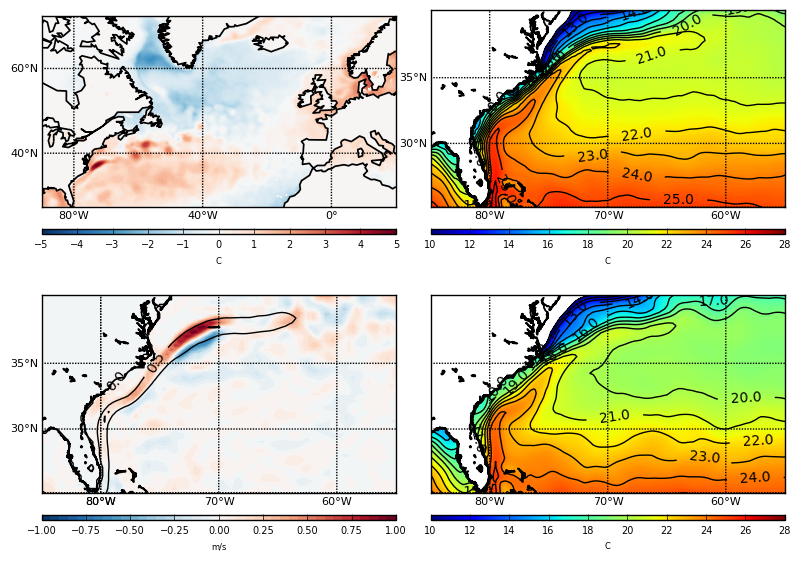
\includegraphics[width=24pc]{sst_current_subplot.png}
	\caption{a) Difference in SST between positive NAO and negative NAO years. b) SST distribution  in positive and d) negative NAO years. d) Difference in surface currents NAO positive - NAO negative. Contour line mean 0.5m/s? current over all winters (2009-10 to 2016-17). SST data from hourly ERA5 reanalysis. Surface current data from OSCAR, 5-day temporal resolution. Seasonal mean (DJF)}
	\label{fig:subplot1} 
\end{figure}

ARGO temperature composite - reinforce the coupled nature of the problem and the importance of ocean dynamics.

I’ve had a quick look at the composite NAO+ minus NAO- in the ARGO climatology of Roemmich and Gilson. The figures attached show meridional sections in the western Atlantic for temperature and salinity. In both, the black contour is the mean and the color the anomaly. You can see the shallow signature of the warmer temperature (and fresher salinity) which is the signature of the SST tripole in this part of the Atlantic. But one can clearly see a temperature anomaly extending deeper (warmer and saltier) around 37N which seems to me to represent a poleward shift of the mean temperature/salinity front. This gives support to the extension of the Gulf Stream suggested by Alison’s SST maps based on OSTIA.


\todo{ this visualization shows OSCAR data - it is not as fast as expected?. Searching for max u or v value in whole dataset over this domain, get ~ 1m/s. When calculate uv, will give 1.4 as the total possible max current. Then I am averaging over season and multiple years, so I guess 0.5 seems reasonable, Check SST STDDEV }
%Mean 1.8, Max speed 2.5m/s but mean over 8 winters is 0.5m/s - this okay?
%https://svs.gsfc.nasa.gov/cgi-bin/details.cgi?aid=3958

%Introduce the fact that here have looked at SST, but the rest of the analysis is looking at mesoscale signatures in the atmosphere and suggest these may be related to the SST.
\todo{Sort references here. Added Cayan but not yet read this paper. Visbeck et al 2000  2003?}

Many studies have examined air-sea interactions associated with western boundary currents  \citep{ma2015distant, shaman2010air, kwon2010role, czaja2001observations, czaja2002observed, minobe2008influence, smirnov2015investigating, kelly2010western, cayan1992latent}, and it has been shown that the Gulf Stream plays an important role in the climate of the northern hemisphere, mainly through affecting the eddy driven jet and associated extra-tropical cyclones \citep{sampe2010significance, nakamura2008importance, booth2012sensitivity, small2014storm, woollings2012response, vanniere2017contribution, vanniere2017cold}. Further to such work on large-scale signals, the focus of this study is to examine whether there also exists a mesoscale signature in the atmosphere as has been shown in the ocean (figure \ref{fig:subplot1}). This is being investigated by analyzing variables smaller than 100 km, reflecting processes that are occurring within the synoptic scale extra-tropical cyclones.

In this study, we use high resolution reanalyses to examine buoyancy and shear production, as well as SST and surface currents during boreal winter and establish whether there exists a relationship with NAO phase. We show that there are mesoscale signals in the NAO in both the atmosphere and the ocean and propose/suggest air-sea interaction.... The paper is organized as follows: section 2 describes the data and methodology used for the analysis. Section 3 shows the spatial distribution of production metrics in ERA5 for different NAO phases, followed by discussion and conclusions in section 4.


%Suggestions that synoptic scale could feed back onto large-scale. What about mesoscale 
%(To analyse the mesoscale signature in both the ocean and atmosphere, to assess air-sea interactions and they relationship with the NAO.
%Furthermore, by comparing two reanalysis datasets, allows assessment into the role of model resolution on this process.)
%We show that there is a signal and propose that this is related to the Gulf Stream warm tongue.

%It is well established that many forecast busts over Europe are due to poor representation of atmospheric blocking \cite{rodwell2013characteristics}.

%It has been suggested (Woollings, etc) that the NAO is related to negative PV, and this study is motivated by Sheldon to examine if this shear diagnostic has a signal in the NAO.

%Further investigation into the effect of the SST on shear instability in these reanalysis products.
%Observational study using reanalyses

%intensity or amount or strength

%\citet{minobe2008influence} found that it affects the entire troposphere. 
%\citep{czaja2011new} - oceans influence the atmopshere through convection in midlatitudes, which is commonly occurring in Tropics.
%ocean on atmosphere in mid-lats, rather than atm on ocean. 

%Current generation weather and climate models are too coarse to properly represent all of the features within in extra-tropical cyclone, and such features are routinely parametrised. Convective instability is included in these schemes and arises from thermal differentials within the atmospheric column. Shear instability is also present, but is not parametrised nor resolved. SI is a shear instability, drawing its energy from 

%The atmosphere may be inertially stable to horizontal displacements and gravitationally unstable to vertical displacements, but may be unstable to slantwise displacements by shear instability. It has been suggested that slantwise convection from the release of (moist symmetric)shear instability can explain banded precipitation often seen at cold fronts \citep{bennetts1979conditional, seltzer1985possible, emanuel1983lagrangian, emanuel1983assessing, morcrette2006formation, chen2018assessment}, caused by cells of alternating rotation creating updrafts and downdrafts.

%Much analysis with ERA-Interim, but new ERA5 is higher resolution with other model improvements.

%Atmospheric reanalyses are a valuable tool for weather and climate analysis and are often treated as the best-guess truth. New improved reanalyes are released generally at increased resolution with other improvements such as to the data assimilation scheme and parametrisations.

%warm conveyor belts

%Shear (or symmetric) instability is a combination of gravitational and inertial instability. A parcel may be inertially stable to horizontal displacements and gravitationally stable to vertical displacements, but may be unstable to slantwise displacements by shear instability. The  M-$\theta$e relationship states that if the $\theta$e surfaces are steeper than the M surfaces, there is symmetric instability. Any slantwise displacement occurring between the slopes of these surfaces will release the symmetric instability and the parcel will be accelerate in the direction away from the original position. Only moist slantwise instability occurs in the Earth's atmosphere \citep{bennetts1979conditional} and so $\theta$e is used. This instability has a 2D assumption that there is no variation in the along front direction.

% 2D theory \citet{eliassen1962vertical}
%%%%%%%%%%%%%%%%%%%%%%%%%%%%%%%%%%%%%%%%%%%%%%%%%%%%%%%%%%%%%%%%%%%%%%%%%%%%%%%%

\section{Data and Methodology}

We use two reanalysis datasets produced by ECMWF (European Centre for Medium-Range Weather Forecasts). ERA-Interim spans 1979-present and has a spatial resolution of 0.75$^{0}$ \citep{dee2011era}. The new ERA5 reanalysis is the 5th major global reanalysis produced by ECMWF and has a finer resolution of 0.25$^{0}$ alongside other model improvements, including increased temporal resolution (ref). The period analyzed is December, January and February, for 5 positive NAO and 2 negative NAO years. The selection of positive and negative NAO years was made using NAO Index Data provided by the Climate Analysis Section, NCAR, Boulder, USA, Hurrell (2003). From 2008 to 2017, when both the station and principal component time series data of sea level pressure agree on sign of NAO index, this year was selected. The 5 positive NAO years (2011-12, 2013-14, 2014-15, 2015-16, 2016-17) and 2 negative NAO years (2009-10, 2010-11) are independent.
%Updated regularly. Accessed DD Month YYYY [list date you accessed the data].

%  %%% get an error about too many brackets when have two tables following each other
% % hyphen is two dashes

  \begin{table}
  \caption{NAO positive and negative winters} \label{t_NAO}
  \centering
  \begin{tabular}{c c c c c c}
  \hline
  \textbf{Positive} & 2011--2012 & 2013--2014 & 2014--2015 & 2015--2016 & 2016--2017 \\
  \hline
  \textbf{Negative}  & 2009--2010  & 2010--2011 &  &  &  \\
  \hline
  \end{tabular}
  \end{table}

%Across each winter, there are 2184 (+x for leap year) time steps. (mean this)

% \begin{figure}[h]
% 	\centering
% 	\includegraphics[width=26pc]{NAO_TS_scatter_norm.pdf}
% 	\caption{DO NOT NEED IN PAPER. NAO}
% 	\label{fig:NAO_TS}
% \end{figure}

The diagnostics are production terms for mesoscale kinetic energy. A spatial filter over a region of 3 degrees (\textasciitilde{300} km) was applied to the data to obtain the high-pass prime values and low-pass bar values, covering 13 and 5 grid points for ERA5 and ERA-Interim, respectively. This is to separate the low frequency background from the high frequency perturbations and to examine small scale has an effect on the large scale. 

\begin{equation} \label{eq_diag1}
\frac{\partial}{\partial{t}} \Bigg(\frac{\overline{u'^2 + v'^2}}{2}\Bigg) = \text{Shear production + Buoyancy production} + ... 
\end{equation}

\begin{equation} \label{eq_diag2}
\text{Shear production} \,(mWkg^{-1}) = -\Bigg({\overline{w'u'} . \frac{\partial{\overline u}}{\partial z} + \overline{w'v'} . \frac{\partial{\overline v}}{\partial z}}\Bigg)
\end{equation}

\begin{equation} \label{eq_diag3}
\text{Buoyancy production} \,(mWkg^{-1}) = {-\overline{w'\alpha'}}
\end{equation}

2-Data and methodology: fine. Don’t forget the BP term in your MKE equation is for pressure coordinate.

% \begin{equation} \label{eq_diag2}
% \frac{\partial}{\partial{t}} EKE = {\underbrace{-\overline{w'u'} . \frac{\partial{\overline u}}{\partial z} + \overline{w'v'} . \frac{\partial{\overline v}}{\partial z}}_{\mathclap{\text{shear instability}}}} {\underbrace{-\overline{w'\alpha'}}_{\mathclap{\text{buoyancy}}}} + ... 
% \end{equation}
%\usepackage{mathtools} % for mathclap
% https://tex.stackexchange.com/questions/36153/annotating-individual-math-terms-with-braces/36154?utm_medium=organic&utm_source=google_rich_qa&utm_campaign=google_rich_qa

Buoyancy is calculated using specific volume ($\alpha$), defined using density from temperature, and u, v, and w, represent zonal, meridional and vertical velocities. Remaining terms denoted by ellipsis include friction. (Averages over DJF are averaged again to give NAO+ and NAO-.)

Twelve pressure levels were used for this analysis (200, 300, 400, 500, 600, 700, 800, 850, 875, 900, 925, 950 hPa), with the lowest and highest omitted from the shear diagnostic calculation as they require another level from which to calculate the shear term. Values are then interpolated (linearly) to every 25 hPa, giving 31 levels in total, and 26 for shear production. In this analysis, integration across levels 300-600 hPa and 625-925 hPa are classified as upper and lower levels, respectively. When integrated across levels (multiplied by dp/g * 1000) both production terms have the units Wm$^{-2}$. 

The SSTs used in both ERA5 and ERA-Interim for the period (2008-present) are from the Operational Sea Surface Temperature and Sea Ice Analysis (OSTIA), which has a resolution of 0.05$^{0}$ \citep{donlon2012operational}. OSCAR (Ocean Surface Current Analysis Real-time) \citep{Bonjean2002} contains near-surface ocean current estimates, on a 0.33$^{0}$ grid. The temporal resolution of variables used from ERA5, ERA-Interim and OSCAR are 1-hourly, 6-hourly and 5-day, respectively.

%However, all these studies were limited to one ora few single events rather than a climatology and the systematicpresence of negative PV in the cold sector has, to our knowledge,never been explored. Negative PV in the cold sector of baroclinicstorms may have received little attention, because it is not includedin classical models of cyclogenesis (e.g. the Eady model has PVequal to 0 uniformly) and because anomalous PV is more oftendiagnosed than PV itself.

%https://podaac.jpl.nasa.gov/dataset/OSCAR_L4_OC_third-deg

%The horizontal velocity is directly estimated from sea surface height, surface vector wind and sea surface temperature.

%(The variables are instantaneous, defined as from the last model time step (ref ECMWF), which is 30 minutes in ERA-Interim and 15 minutes in ERA5.)

% ERA5 uses the same 37 pressure levels as ERA-Interim.
%The instability in the x (u) and y (v) directions are combined. The covariance of small-scale vertical motions ($\omega$') and horizontal vertical motions (u' or v') is calculated and then the  product with the vertical shear of low pass winds ($\overline{u}$ or $\overline{v}$)  is created. The high pass, to capture the high variability, was original minus low pass. 
%computed over the North Atlantic domain (20-80N, 90W-40E).

%Negative potential vorticity has been analysed in the ERA5 dataset as this is output from the model. Only PV that is negative has been analysed.

%Although the atmospheric model resolution is constant throughout the whole data set, the prescribed SST data has changed. ERA-Interim data is analysed from 2002-2018, when the SST resolution is at least as fine as the atmospheric resolution. In years prior to this, the SST is coarse and ....
%ERA5 uses SSTs from HadISST version 2 0.25$^{0}$(Kennedy et al. 2016) to 2007, and thereafter OSTIA 0.05$^{0}$.
%ERA-Interim SST change and effect on air-sea interaction \citet{parfitt2017impact}
%Late 2018	Complete the release of 1979-2009
%Just compare ERA-Interim with ERA-5. For a fair comparison, use ERA5 at same time resolution as ERA-Interim

%%%%%%%%%%%%%%%%%%%%%%%%%%%%%%%%%%%%%%%%%%%%%%%%%%%%%%%%%%%%%%%%%%%%%%%%%%%%%

\section{Results}


3.1 Upper ocean: describe SST, OSCAR: show that there is more than the SST tripole. Probably good to use Sheldon et al results here to motivate the use of SP, BP and “anchoring” idea.
3.2 Mesoscale diagnostic in the atmosphere: first say we recover the standard north-south dipole in classic variables such as U at 300hPa or EKE (probably not showing it, this is not new). Then describe BP and SP with emphasis on the SW-NE dipole embedded in the large scale NorthSouth shift.

Results shown are positive production terms (equations \ref{eq_diag2}, \ref{eq_diag3}) calculated from hourly ERA5 reanalysis data over the winter season (DJF), averaged over the years in each NAO phase. The warm tongue is narrower and warmer in NAO+, with the 21 $^{0}$C isotherm approximately collocated with the 20 $^{0}$C isotherm (figure \ref{fig:subplot1}). The 21 $^{0}$C isotherm is shown in figures \ref{fig:ERA5_buoy} and \ref{fig:ERA5_shear}.

In NAO+, the magnitude of buoyancy is approximately 20\% higher in the lower atmosphere (600-925 hPa) than the upper atmosphere (300-600 hPa), whereas in NAO- the magnitude is more consistent (figure \ref{fig:ERA5_buoy}). This reflects the more extensive presence of warm water, opposing the expectation from more cold air outbreaks in NAO-. The intensity between NAO phases is similar, however the spatial distribution shows differences, with an increase at higher latitudes and decrease in lower latitudes in NAO+. This is the expected shift of synoptic activity with NAO phase. At low levels in NAO+, over the Gulf Stream there is a displacement of buoyancy northeastwards along the warm tongue, suggesting an anchoring of this production term by the warm tongue.

%The heat loss in the Labrador Sea in the positive NAO years is consistent. 
%The lower atmosphere more intense than the upper atmosphere, 

\begin{figure}[h]
	\centering
	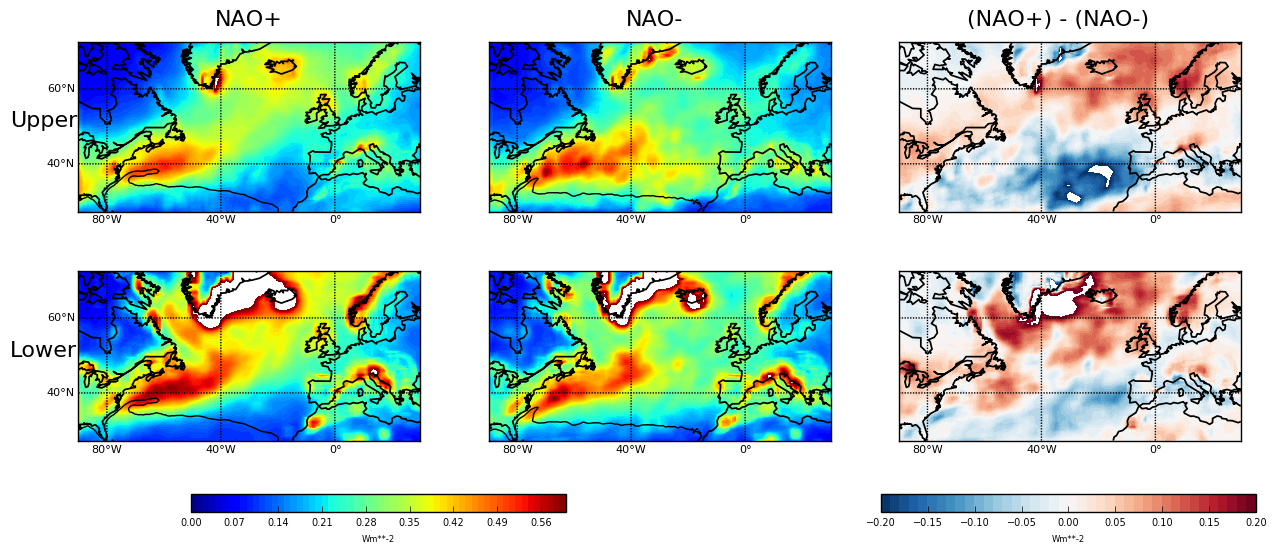
\includegraphics[width=32pc]{ERA5_6buoy_subplot2.pdf}
	\caption{Distribution of positive buoyancy integrated over the upper atmosphere (300-600 hPa) in (a) positive (b) and negative NAO phases and the lower atmosphere (625-925 hPa) in (d) positive (e) and negative NAO phases. Difference in integrated positive shear production NAO positive-NAO negative in the (c) upper atmosphere and (f) lower atmosphere. The 21 $^{0}$C SST isotherm is shown in black contours. At positive saturation, white is shown.}
	\label{fig:ERA5_buoy}
\end{figure}

\todo{Look at surface fluxes? Cold air or warm water dominant?}
%%%%%%%%%%%%%%%%%%%%%%%%%%%%%%%%%%%%%%%%%%%%%%%%%%%%%%%%%%%%%%%%%%%%%


%The lower atmosphere more intense than the upper atmosphere.
%In positive NAO years, the UK and Norway experience higher values of positive shear production.
For the shear production term, a zonal extension is observed in NAO-, especially in the upper atmosphere (figure \ref{fig:ERA5_shear}), consistent with the pattern of buoyancy. Shear production is approximately 25\% weaker than buoyancy. Over the warm tongue region, shear production is displaced further northeast in NAO+, along the axes of the extended warm tongue. The largest values of shear production are over high orography, particularly Greenland, where white is color bar saturation. Away from these regions, the most intense values are downstream of the warm tongue, where there is also the maximum difference in the lower atmosphere. More spread downstream in the upper atmosphere. This zonal flow in NAO- can be seen in the time mean large-scale EKE at 200 hPa (figure \ref{fig:ERA5_EKE200_NAO} supplementary), which is a proxy for the storm track.

%In the lower atmosphere, that amplitude of the instability is comparable to in the upper atmosphere and the difference between NAO phases shows the same broad pattern, with slightly reduced difference in magnitude. 

\begin{figure}[h]
	\centering
	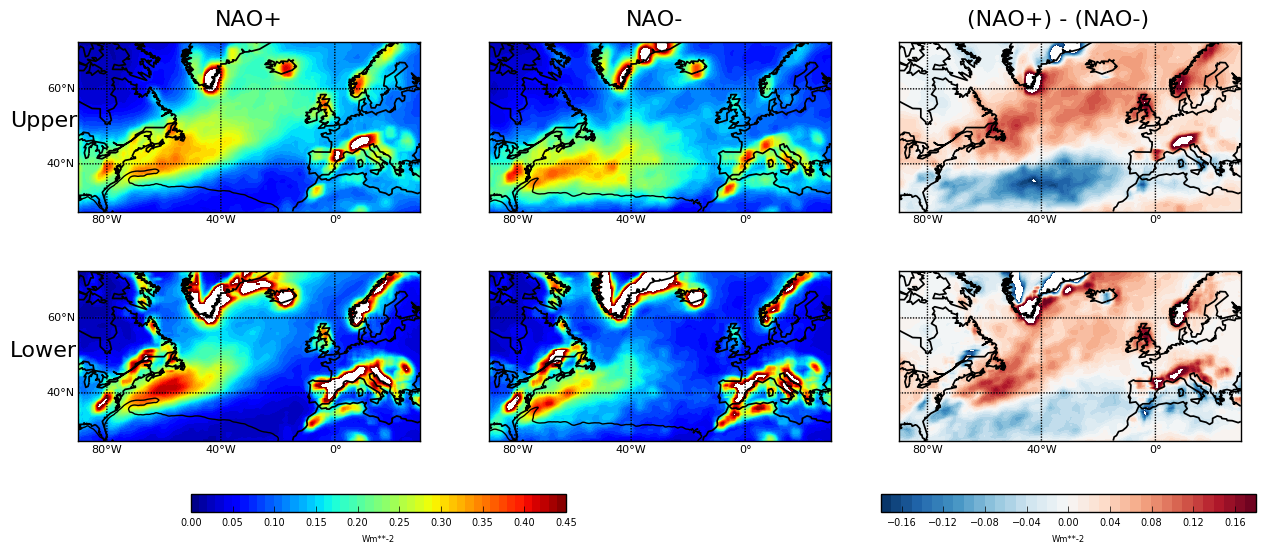
\includegraphics[width=32pc]{ERA5_6shear_subplot2.pdf}
	\caption{Distribution of positive shear production integrated over the upper atmosphere (300-600 hPa) in (a) positive (b) and negative NAO phases and the lower atmosphere (625-925 hPa) in (d) positive (e) and negative NAO phases. Difference in integrated positive shear production NAO positive-NAO negative in the (c) upper atmosphere and (f) lower atmosphere. The 21 $^{0}$C SST isotherm is shown in black contours. At positive saturation, white is shown.}
	\label{fig:ERA5_shear}
\end{figure}


The vertical distribution of buoyancy and shear production is relatively homogeneous throughout the troposphere, with peaks around 500 400 hPa.

%%%%%%%%%%%%%%%%%%%%%%%%%%%%%%%%%%%%%%%%%%%%%%%%%%%%%%%%%%%%%%%%%%%%%


% \begin{figure}[h]
% 	\centering
% 	\includegraphics[width=20pc]{ERA5_PVneg_hist_log_NAOneg_300_600_925.pdf}
% 	\caption{Distribution neg PV NAO neg}
% 	\label{fig:ERA5_PV_dist_NAOneg}
% \end{figure}

% \begin{figure}[h]
% 	\centering
% 	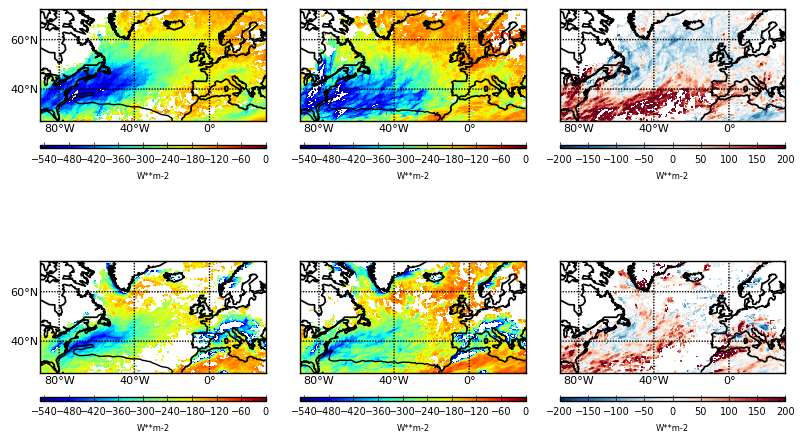
\includegraphics[width=40pc]{ERA5_6PV_mean_subplot.png}
% 	\caption{CHOOSE EITHER MEAN NEG PV OR NEG PV COUNT. Distribution of mean negative PV in the upper atmosphere (300-600 hPa) in (a) positive (b) and negative NAO phases and in the lower atmosphere (625-925 hPa) in (d) positive (e) and negative NAO phases. Difference in  mean negative PV NAO positive-NAO negative in the (c) upper atmosphere and (f) lower atmosphere. The 21 $^{0}$C SST isotherm is shown in black contours. At positive saturation, white is shown.}
% 	\label{fig:ERA5_PV_mean}
% \end{figure}

% \begin{figure}[h]
% 	\centering
% 	\includegraphics[width=14pc]{ERA5_PV_stack_subplot_NAOneg.pdf}
% 	\caption{SHOW EITHER NAO POS OR NAO NEG OR SUM OF ALL YEARS. Multi layer contour plot of negative PVU count for positive NAO years DJF from hourly ERA5 data.}
% 	\label{fig:ERA5_PVU_NAOneg}
% \end{figure}

% \begin{figure}[h]
% 	\centering
% 	\includegraphics[width=10pc]{GS_stack_ERA5_shear_diag_DJF_pos_mean_NAOneg.pdf}
% 	\caption{Multi layer contour plot of negative shear diag for positive NAO years DJF from hourly ERA5 data.}
% 	\label{fig:ERA5_PVU_shear_diag_layer_NAOpos}
% \end{figure}

%%%%%%%%%%%%%%%%%%%%%%%%%%%%%%%%%%%%%%%%%%%%%%%%%%%%%%%%%%%%%%%%%%%%%

The same analysis conducted with ERA-Interim 6-hourly data revealed the same spatial pattern in buoyancy and positive shear production with NAO phase, but with differences in magnitude. In ERA-Interim, the values as well as differences of shear and buoyancy production approximately halved. Expected in a coarser resolution model. By definition of these diagnostics (equations \ref{eq_diag2}, \ref{eq_diag3}) and the region size over which the bars and primes are calculated (3 degrees), there will be more production in ERA-5, where 13 grid points have been used, whereas only 5 are used in ERA-Interim.
Three times coarser but only twice as weak?? ERAI uses 6-hourly vs hourly in ERA5!

%%%%%%%%%%%%%%%%%%%%%%%%%%%%%%%%%%%%%%%

\section{Discussion and conclusions}

We motivate this study by showing a mesoscale signature in SST and surface currents with NAO phase. While previous studies have examined the NAO large-scale tripole in SST, this new high resolution reanalysis allows us to describe a smaller scale feature embedded within. We then show that there is a signal in atmospheric buoyancy and shear production aligned with the storm track on the large scale, and also a more localized relationship with NAO phase over the warm tongue region.

%At a localized scale over the Gulf Stream warm tongue, the production terms are displaced in NAO phase in relation to the warm tongue structure \todo{see final new plot}
%%%%%%%%%%%%%%% PV %%%%%%%%%%%%%%%%%%

\begin{figure}[h]
	\centering
	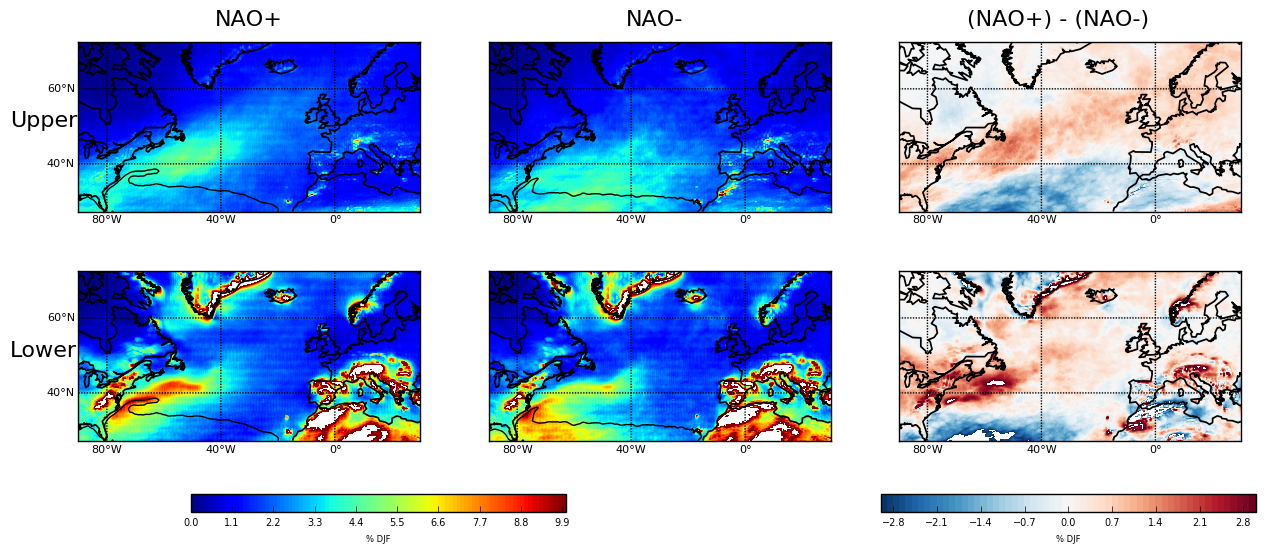
\includegraphics[width=32pc]{ERA5_6PV_subplot2.pdf}
	\caption{Frequency (percentage of DJF) of negative PV averaged over the upper atmosphere (300-600 hPa) in (a) positive (b) and negative NAO phases and averaged over the lower atmosphere (625-925 hPa) in (d) positive (e) and negative NAO phases. Difference in frequency of negative PV NAO positive-NAO negative in the (c) upper atmosphere and (f) lower atmosphere. The 21 $^{0}$C SST isotherm is shown in black contours. At positive saturation, white is shown.}
	\label{fig:ERA5_PV_count_cent}
\end{figure}

Analysis of negative PV because...
Figure \ref{fig:ERA5_PV_count_cent} shows the frequency (as percentage of DJF) of occurrence of negative potential vorticity averaged over upper and lower levels. \citet{vanniere2016potential} showed that negative PV generated within the cold sector of extra-tropical storms is present (GS region?) approximately 10-12\% of the time. I GUESS I DO NOT WANT TO SAY THAT THIS IS CONSISTENT WITH MY PLOT. MY PLOT IS MEAN OVER MULTIPLE LEVELS AND IS ACTUALLY MUCH LARGER WHEN LOOK AT STACKED PLOT. In the upper atmosphere this is 3-4\%, and in the lower atmosphere is approximately double, frontal occurrence, rapid ascent. We observe the smaller scale signal at low levels, with 'downstream anchoring’ effect of the warm tongue. The presence of negative PV in the upper atmosphere over land is absent, whereas there was strong positive shear production. This suggests that the shear production was mountain wave drag over regions of high orography.

Figure \ref{fig:ERA5_PV_count_cent} shows relatively frequent negative PV at low latitudes and across much of the western part of the Atlantic basin in NAO-. This will be investigated in future?

\begin{figure}[h]
	\centering
	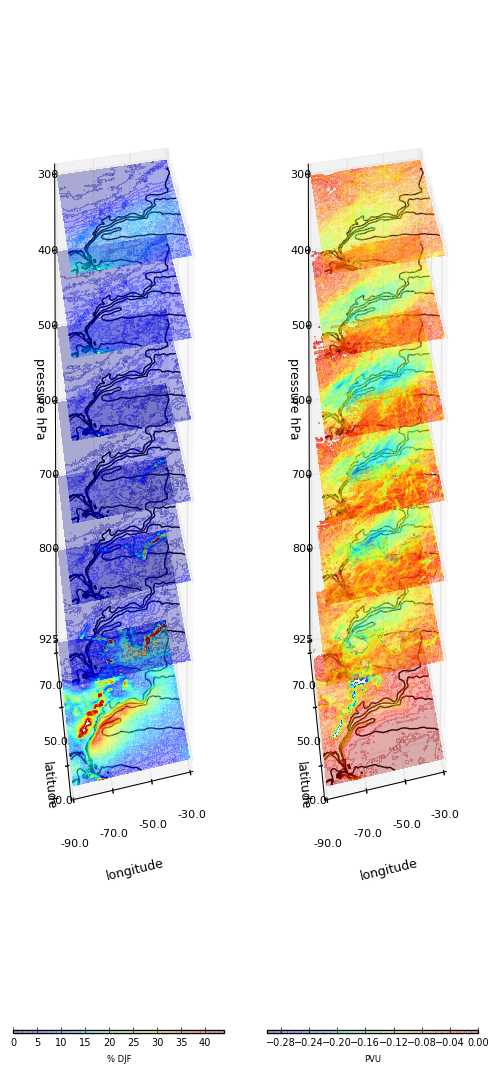
\includegraphics[width=14pc]{ERA5_PV_stack_subplot_NAOpos.pdf}
	\caption{Stacked contour plot of a) negative PV frequency and b) mean negative PV at 925, 800, 700, 600, 500, 400, 300 hPa with SST contour lines.}
	\label{fig:ERA5_PV_stack}
\end{figure}

% \begin{figure}[h]
% 	\centering
% 	\includegraphics[width=14pc]{ERA5_PVneg_hist_log_NAOpos_300_600_925.pdf}
% 	\caption{POSSIBLY COMBINE HISTOGRAM IN SUBPLOT WITH STACKED PLOT. Distribution neg PV NAO pos. 80-40W 30-60N}
% 	\label{fig:ERA5_PV_dist_NAOpos}
% \end{figure}

The high frequency of negative PV in the lower levels is dominated by that at 925 hPa (figure \ref{fig:ERA5_PV_stack}, NAO+). The southeastward advection of continental air over the ocean by an extra-tropical cyclone will generate a cold air outbreak, and production of negative PV, but not all storms generate a front large enough to be counted by the frontal detection studies. This stacked plot shows the same vertical structure in the NAO negative years. Throughout the rest of the troposphere, the frequency is consistently lower, but with a relative increase at the 300 hPa. The mean value of negative PV at each layer shows the opposite pattern, with largest magnitude in the mid layers. Strong ascent required to bring the PV all the way to 300hPa are much less frequent than the cold air outbreak. The middle layers hardly keep track of this because of fast ascent, while the spreading at upper levels allow it to be seen there. (Talk about histogram distribution (not shown)?)

%In summary, this observational study using a modern reanalysis suggests the possibility of a positive feedback between the ocean on the NAO on scales smaller than those having been discussed so far in the literature.

\begin{figure}[h]
	\centering
	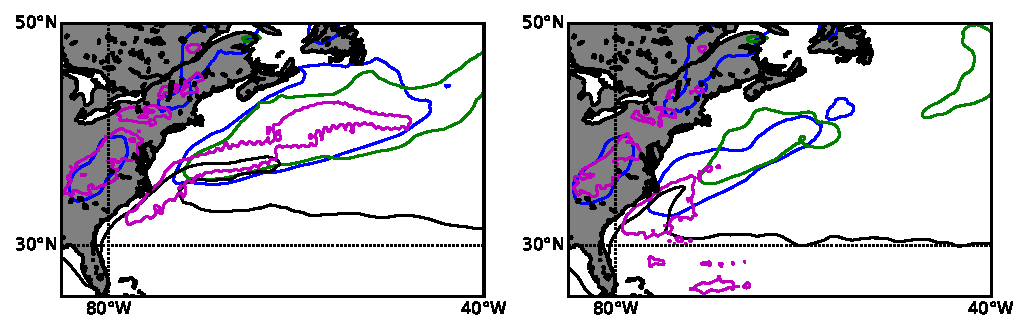
\includegraphics[width=30pc]{Sub_overlay_GS.pdf}
	\caption{a)NAO+ b)NAO-. SST (black), PV (magenta), Shear, Buoyancy. Single contour of each variable. Maybe put in supplementary or delete}
	\label{fig:ERA5_overlay}
\end{figure}


%%%%%%%%%%%%%%%%% Sheldon %%%%%%%%%%%%%%%%%%%%%%%%

In an modeling study using a 12 km grid, \citet{sheldon2017warm} showed that the Gulf Stream warm tongue affects atmospheric shear production.  When a strong Gulf Stream warm tongue was present, shear production was found downstream, but in an experiment where the SST is smoothed, the shear production is reduced (figures \ref{fig:Sheldon}). Along with this signal in shear production, they found a region of negative PV at mid-levels associated with the warm tongue, and lack of this in a smooth set up. Alongside this study it suggests that the SST warm tongue anchors shear production - but also buoy?? need buoy to get shear?

\begin{figure}[h]
	\centering
	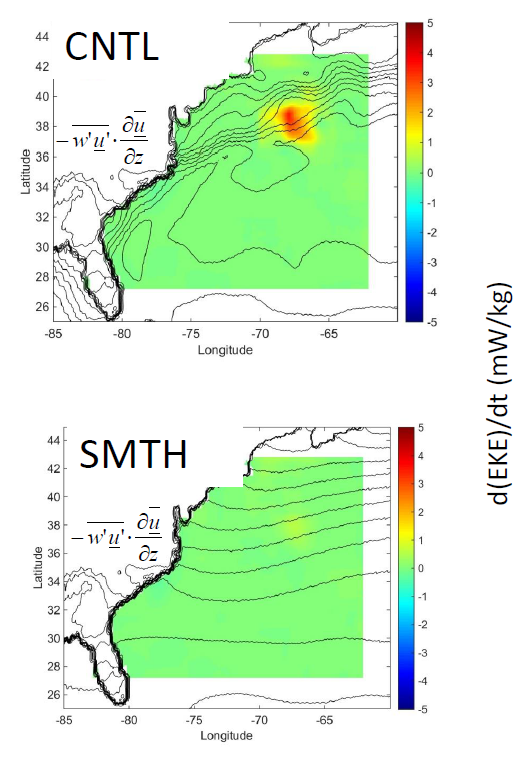
\includegraphics[width=14pc]{Arnaud_plot.PNG}
	\caption{Distribution of shear production (in mW/kg) at height z=4.5 km 24 hours into the model run. (a) control (b) smooth. The associated SST distributions are shown in black contours. Further work from analysis \citet{sheldon2017warm}.}
	\label{fig:Sheldon} 
\end{figure}

This hypothesis warrants further investigation through a modeling study at high resolution (at least 0.25$^{0}$) run for climatological time scales to examine the causal relationships between these two variables... Experiment isolate the mechanism


%%%%%%%%%%%%%%%%%%%%%%%%%%%%%%%%%%%%%%%%%%%%%%%%%%%%%%%%%%%%

The SST front has a substantial impact on the marine atmospheric boundary layer above - how? wind convergence over sst gradient (Chelton et al., 2004).

Thought confined to boundary layer, but can see throughout troposphere - can we see this in ERA-I?

4-Discussion: First thing is our interpretation in terms of passive / active, motivated by the expts in Sheldon et al. To support this further discuss the PV maps. Then a few specific issues:
*SST pattern: possibly we’re seeing something quite different from previous studies (de Coetlogon and Frankignoul, 2001; Sasaki et al., 2011) because of the persistent NAO+ conditions since ~2010.
*short dataset
*…
5-Conclusion: come back to the initial question and answer: yes, the new datasets show that there is something else going on with NAO, not just the SST tripole and north south shift of the storm track-jet. Our study has established this, now key issue is whether it matters for the NAO and for seasonal to decadal prediction. We can then speculate about mechanisms of feedback onto the NAO (I’m thinking PV<0 is injected at the right place in NAO- to sustain more frequent blocks but we’ll need to see your NAO PV maps to say)

In summary, this analysis shows the presence of mesoscale signatures in the NAO, with the atmospheric feature anchored downstream of that in the ocean. This is the southwest-northeast dipole that is so clear in figures \ref{fig:ERA5_buoy} and \ref{fig:ERA5_shear}. We suggest that this relationship between the atmosphere and  Gulf Stream warm core is 'active', based on results from \citet{sheldon2017warm}, in contrast to the 'passive' mesoscale signal of the large-scale shift of storm track. Highlights the importance of high resolution, able to resolve.../represent... mesoscale... ERA-I and ERA5 have same, high resolution SST, but different atmosphere. Too fine for them, especially ERA-I.

Isla Simpson: recent paper:
"While the above analysis leads us to conclude that the multi-decadal variabilty in March U700 504 is most strongly connected with the AMV, some ambiguity remains over the causal nature of this 505 connection. It is well known that variability in the North Atlantic atmospheric circulation and 506 associated surface fluxes is, itself, a driving force for North Atlantic SST variability (Deser and 507 Blackmon 1993; Deser et al. 2010), whether it be through the influence on the deep ocean circula508
tion (Eden and Jung 2001; Danabasoglu et al. 2014; Yeager and Danabasoglu 2014; Delworth and 509 Zeng 2016; Delworth et al. 2017) or direct influence on the ocean mixed layer (Seager et al. 2000; 510 Clement et al. 2015; Cane et al. 2017). It is, therefore, plausible that these connections indicate 511 a causal link in the opposite sense i.e., the multi-decadal variability in the winds is driving the
512 multi-decadal variability in the SSTs. While the coupling between ocean and atmosphere likely 513 goes both ways, we summarize here various lines of reasoning  that support a directed causal link 514 between the SST variability and March U700 in the sense of the SSTs driving March U700.
The conventional view of North Atlantic ocean-atmosphere coupling, however, is that the pri624
mary direction of interaction is the opposite of this, with the winds influencing the SSTs. Evidence
625 for a connection in the other direction, during winter, is somewhat patchy. It has been argued that North Atlantic SST variability may influence the North Atlantic jet
694 through a stratospheric pathway (Omrani et al. 2014).  Indeed,
707 recent studies have suggested that improved resolution of ocean fronts and the overlying atmo708
sphere could significantly alter the nature of ocean-atmosphere coupling (Smirnov et al. 2015;
709 Parfitt et al. 2016; Siqueira and Kirtman 2016)."

Visbeck chapter: "However, outside of the deep
tropics, most studies find that the ocean largely reacts to the high frequency changes of the
atmospheric forcing and that its influence back to the atmosphere is weak on time scales shorter
than a decade."

Bishop: ocean weather

shear instability = barotropic?

\todo{Things to mention: significance, short 5 \& 2 years analysis, heat flux, geostrophy, feedback on large scale, ocean-atmosphere coupling in the mid-latitudes, mesoscale.}
\todo{Visbeck, Sasaki, Marshall, Cassou, Fan \& Schneider, Small, Bryan, Rodwell, Peng, Wang, Ma, Czaja.}

%Why does shear production not also happen in this region where there are warmer waters in the positive phase? need some buoyancy to get shear? look at relationship / correlation between buoyancy and shear. too stable over warm waters, do not get shear production either?
% novel approach
%entirely consistent with a feedback
%Negative PV has been reported in the cold sectors of extratropical cyclones (Stoelinga, 1996; Chagnon et al., 2013). Chagnon et al. (2013)showed that negative PV arose from the boundary-layer tendencyand was generated by strong positive heat flux (maximum atthe surface).
%In boreal winter, cold air outbreaks are common in the Western North Atlantic, leading to large heat transfer as this air passes over the warm waters of the Gulf Stream (Zolina and Gulev, 2003).


%%%%%%%%%%%%%%%%%%%%
Supplementary material: figure \ref{fig:ERA5_EKE200_NAO}

\begin{figure}[h]
	\centering
	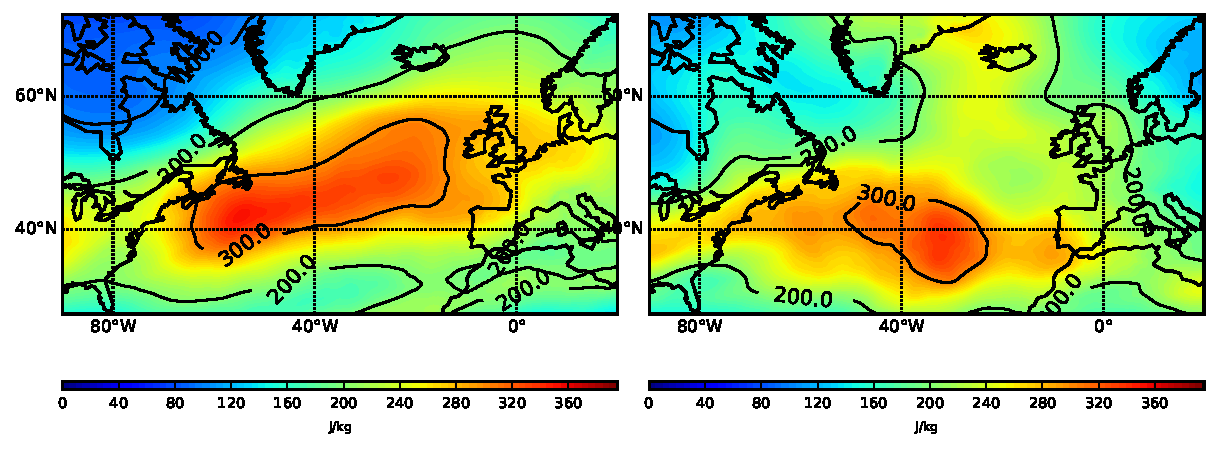
\includegraphics[width=20pc]{ERA5_EKE200_subplot.pdf}
	\caption{Large scale time mean EKE at 200 hPa for a) positive and b) negative NAO years from hourly ERA5 data. NEED TO FILTER < 10day}
	\label{fig:ERA5_EKE200_NAO}
\end{figure}

Supplementary material: figure ECMWF shear diagnostic
\begin{figure}[h]
	\centering
	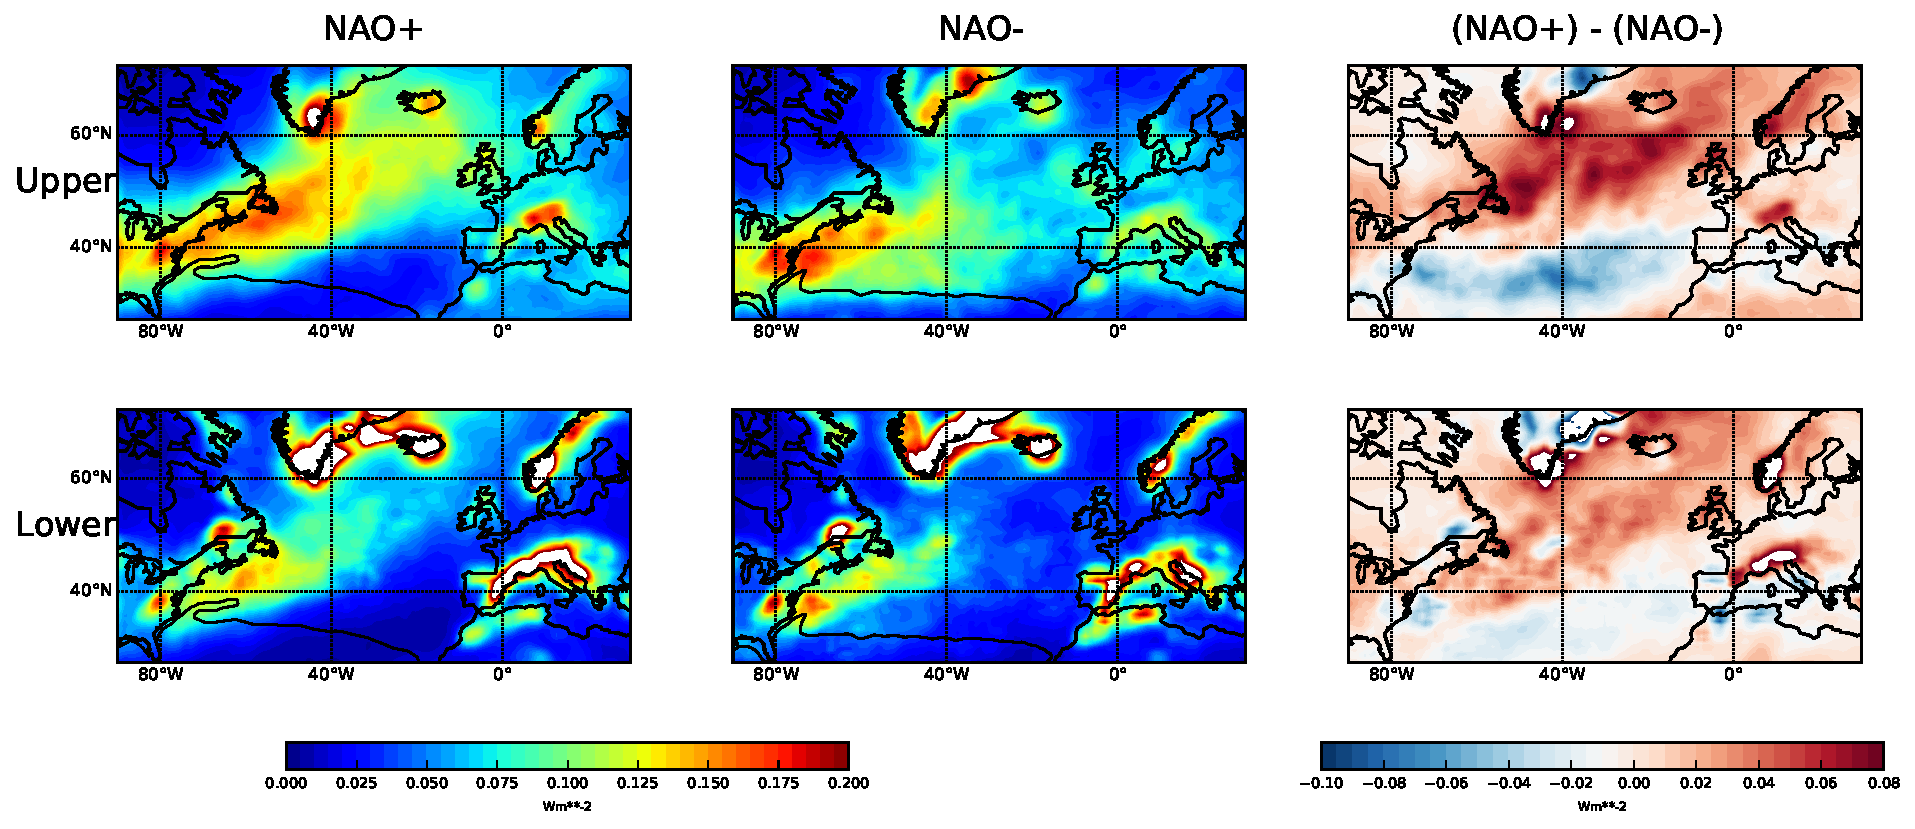
\includegraphics[width=32pc]{ERA_6shear_subplot.pdf}
	\caption{Distribution of positive buoyancy integrated over the upper atmosphere (300-600 hPa) in (a) positive (b) and negative NAO phases and the lower atmosphere (625-925 hPa) in (d) positive (e) and negative NAO phases. Difference in integrated positive shear production NAO positive-NAO negative in the (c) upper atmosphere and (f) lower atmosphere. The 21 $^{0}$C SST isotherm is shown in black contours. At positive saturation, white is shown.}
	\label{fig:ERA_shear}
\end{figure}
%%%%%%%%%%%%%%%%%%%%%%%%%%%%%%
%The \citet{sheldon2017warm} study found a value of approximately 5 mW/kg at 5 km at one time step. Here, the maximum value over the Gulf Stream region is ~ 40 times weaker. There are model difference, including a doubling of resolution in this study from 12 km in Sheldon to 25$^{0}$ in ERA5. Also this result takes an average over 10 levels, which were interpolated from ..., where any positive value was taken into the mean for each phase. Also this analysis over DJF picks up storms at all stages of their life cycle, perhaps when this instability was weaker than in the single Sheldon experiment. Analysis of the distribution of shear instability values revealed that 5mw/kg could be achieved, but with a probability of ..percent. amplitude of anomaly or difference or total value?
%Note that in both my subsets, there is a GS warm tongue (unlike Sheldon experiment, where one is smoothed).

%This upper atmosphere slice included 500 hPa, which is comparable to 5 km, where \citet{sheldon2017warm} found the maximum of shear instability in the vertical. 

%Over the North Atlantic, the dominant mode of atmospheric variability is the NAO, which is associated with a latitudinal displacement of the jet. We find that winters associated with a negative phase of the NAO are related to reduced EKE over the Atlantic (not shown), suggesting that a midwinter minimum is more likely to occur in the Atlantic during years of negative NAO. In our analysis, most years of strong jet are associated with negative NAO in winter (five out of seven), and years of weak jet are associated with positive NAO (six out of seven).

%has a (significantly different) spatial distribution in a high resolution reanalysis depending on NAO state. The positive NAO drives the tripole SST pattern and, we find, also a strengthening of the Gulf Stream warm tongue. Such an SST distribution leads to more shear instability downstream of the warm tongue.


%%%%%%%%%%%%%%

\section{Abbreviations}
%http://tex.stackexchange.com/questions/74353/what-commands-are-there-for-horizontal-spacing

% Acronyms
\begin{acronyms}
	\acro{ECMWF}
	European Centre for Medium-Range Weather Forecasts
	\acro{EKE}
	Eddy Kinetic Energy
	\acro{NAO}
	North Atlantic Oscillation
	\acro{OSTIA}
	Operational Sea Surface Temperature and Sea Ice Analysis
	\acro{OSCAR}
	Ocean Surface Current Analysis Real-time
	\acro{PV}
	Potential Vorticity
\end{acronyms}

\begin{tabular}{ l l }
	AGCM & Atmospheric Global Climate Model \\
	%	D26 & Depth of 26C isotherm \\
	DLM & Deep layer mean \\ 
	%	EASM & East Asian summer monsoon \\
	ENSO & El Ni\~{n}o Southern Oscillation \\ 
	ECMWF & European Centre of Medium--range Weather Forecasting \\
	
	GCM & Global Climate Model Circ model?? \\
	MABL & Marine Atmospheric Boundary Layer \\
	MetUM & Met Office Unified Model \\
	OGCM & Ocean Global Climate Model \\
	%	SSHS & Saffir Simpson Hurricane Scale \\
	SST & Sea surface temperature \\
	
	
\end{tabular}


\newpage



%%%%%%%%%%%%%%%%%%%%%%%%%%%%%%%%%%%%%%%%%%%%%%%%%%%%%%%%%%%%%%%%


\acknowledgments
ECMWF
NAO Index Data provided by the Climate Analysis Section, NCAR, Boulder, USA, Hurrell (2003). Updated regularly. Accessed 17 April 2018.
Magdalena, Frederic, Paul Dando

'Generated using Copernicus Climate Change Service Information [2018]'.
% https://software.ecmwf.int/wiki/display/CKB/ERA5+data+documentation#ERA5datadocumentation-HowtociteERA5

OSCAR citation ESR. 2009. OSCAR third degree resolution ocean surface currents. Ver. 1. PO.DAAC,	CA,	USA. Dataset accessed [YYYY-MM-DD] at http://dx.doi.org/10.5067/OSCAR-03D01.
